\begin{figure}[htp]
	\begin{center}
	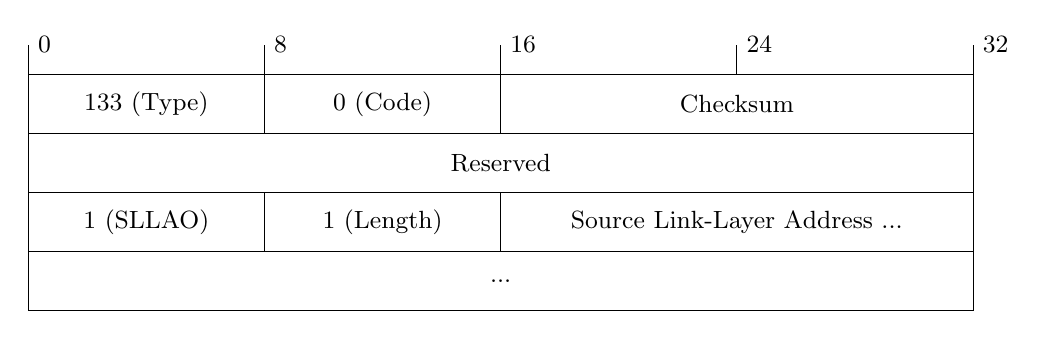
\begin{tikzpicture}[scale=0.75]
		\draw (0,0) rectangle (16,4);
		\draw (0,4) -- ++(0,0.5) node[right] {\small 0};
		\draw (4,4) -- ++(0,0.5) node[right] {\small 8};
		\draw (8,4) -- ++(0,0.5) node[right] {\small 16};
		\draw (12,4) -- ++(0,0.5) node[right] {\small 24};
		\draw (16,4) -- ++(0,0.5) node[right] {\small 32};

		\draw (4,4) -- (4,3);
		\node at (2,3.5) {\small 133 (Type)};
		\draw (8,4) -- (8,3);
		\node at (6, 3.5) {\small 0 (Code)};
		\node at (12, 3.5) {\small Checksum};
		\draw (0,3) -- ++(16,0);

		\node at (8, 2.5) {\small Reserved};
		\draw (0,2) -- ++(16,0);

		\draw (4,2) -- (4,1);
		\node at (2,1.5) {\small 1 (SLLAO)};
		\draw (8,2) -- (8,1);
		\node at (6, 1.5) {\small 1 (Length)};
		\node at (12, 1.5) {\small Source Link-Layer Address ...};
		\draw (0,1) -- ++(16,0);
		\node at (8, 0.5) {\small ...};

	\end{tikzpicture}
	\end{center}
	\caption{Router Solicitation Message Example}
	\label{fig:ipv6_rs}
\end{figure}